%------------------------------Bibliotheken--------------------------------
\documentclass[oneside]{scrbook}
\setkomafont{author}{\scshape}
\usepackage[utf8]{inputenc}
\usepackage{blindtext}
\usepackage{booktabs}
\usepackage{hyperref}
\usepackage{graphicx}
\usepackage{lmodern,textcomp}
\usepackage[toc]{glossaries}
\usepackage{geometry}
\usepackage[dutch]{babel}
\usepackage{listings}
\usepackage{csquotes}
\usepackage{enumitem}
\usepackage{comment}
\usepackage{array}
\usepackage{lipsum}
\setlength{\parindent}{0em}
\setlength{\parskip}{1em}
\graphicspath{{figures/}}
\usepackage[usestackEOL]{stackengine}
\usepackage{tabularx}
\usepackage{adjustbox}
\usepackage{float}
\usepackage[toc,page]{appendix}
\usepackage[T1]{fontenc}
\usepackage{xcolor}

% ---------------------------------------Woordenlijst-----------------------------

\makeglossaries

\def\code#1{\texttt{#1}}

\usepackage[nottoc]{tocbibind} %Adds "References" to the table of contents

\date{\today}

% ------------------------Lijst van figuren--commando---------------------
\renewcommand{\listfigurename}{Lijst van figuren}

% ---------------------------Begin--van--het--document---------------------
\begin{document}

\strutlongstacks{T}

\begin{titlepage} % Suppresses displaying the page number on the title page and the subsequent page counts as page 1
	\newcommand{\HRule}{\rule{\linewidth}{0.5mm}} % Defines a new command for horizontal lines, change thickness here
	
	\center % Centre everything on the page
	
	%------------------------------------------------
	%	Headings
	%------------------------------------------------
	
	\textsc{\LARGE Hogeschool Rotterdam}\\[1.5cm] % Main heading such as the name of your university/college
	
	\textsc{\Large Technische Informatica}\\[0.5cm] % Major heading such as course name
	
	\textsc{\large Tinlab Advanced Algorithms}\\[0.5cm] % Minor heading such as course title
	
	%------------------------------------------------
	%	Title
	%------------------------------------------------
	
	\HRule\\[0.4cm]
	
	{\huge\bfseries Gezamenlijk Eindverslag}\\[0.4cm] % Title of your document
	
	\HRule\\[1.5cm]
	
	%------------------------------------------------
	%	Author(s)
	%------------------------------------------------
	
	{\large\textit{Auteurs}}\\
	Jorian Nakorikantodas 0969032  \\
	Matthijs Meijerink 0962038 \\
	Ebrar Eryigit 0961449 \\*
	Aroena Almeida Mendes 0968262 
        
        
    %------------------------------------------------
	%	School(sc)
	%------------------------------------------------
	
	{\large\textit{School}}\\
    Hogeschool Rotterdam Wijnhaven  \\*
    3011 WN Rotterdam \\*
    Nederland
    
    %------------------------------------------------
	%	Stagebegeleider(st)
	%------------------------------------------------
	
	{\large\textit{Docenten}}\\
    Wessel Oele \\
    Elvira van der Ven
    
    %------------------------------------------------
	%	Vakcode
	%------------------------------------------------
    {\large\textit{Vakcode}}\\
    TINLAA01
    
    %------------------------------------------------
	%	Logo_HR
	%------------------------------------------------
	
	\begin{figure}[H]
    \centering
    
\includegraphics[width=3.7cm,height=3.2cm]{logohr.png}
    \end{figure}
	
	%------------------------------------------------
	%	Date and versionnumber
	%------------------------------------------------
	
	\vfill\vfill\vfill % Position the date 3/4 down the remaining page
	
	{\large\today} \\ % Date, change the \today to a set date if you want to be precise
	{\large\textit{versie}} 1.1\\  % version of the document
	 
	%----------------------------------------------------------------------------------------
	
	\vfill % Push the date up 1/4 of the remaining page
	
\end{titlepage}


%-------------------------------Samenvatting-------------------------------
\chapter{Opdracht}
Onze opdracht is om een sluis te modelleren. We hebben enkele requirements gekregen waarmee we uiteindelijk onze eigen keuzes mogen maken om een sluis te modelleren. Het model moet uitbreidbaar zijn om in meerdere situaties toegepast te kunnen worden. We moeten technische besluiten gaan nemen over het type sluis dat we gaan modelleren, gebruik van sensoren, queues en integers in het model, het aantal boten, tijd en het waterniveau. We zullen deze keuzes ook gaande het verslag beargumenteren.
% --------------------------------Lijst-van-figuren-----------------------
\listoffigures

% ---------------------------------Lijst-van-tabellen------------------------
\listoftables

%-------------------------------Inhoudsopgave------------------------------
\tableofcontents{}

% -----------------------------------------Sluizen--------------------------------

\chapter{Sluizen}
\section{Soorten Sluizen}
Voor onze opdracht hadden we de vrijheid om zelf een type sluis uit te kiezen die we vervolgens moesten modelleren. Er waren verassend veel type sluizen waar we uit konden kiezen:

\begin{itemize}
    \item Zeesluis
    \item De schutsluis
    \item De keersluis
    \item De uitwateringssluis
    \item De ontlastsluis
    \item De inlaatsluis
    \item De spuisluis
    \item De inundatie sluis
    \item De doksluis.
    \item Waaiersluis

\end{itemize}
De sluis die we uiteindelijk hebben gekozen is de schutsluis. We zullen hieronder kort uitleggen waarom deze sluis onze keuze is geweest.

\begin{itemize}
    \item Eenvoudig: Dit type sluis heeft de minste bewegende onderdelen en sensoren. Het modelleren en verifiëren vergt hierdoor minder werk.
    \item Veiligheid: Doordat dit type sluis niet veel onderdelen heeft, is het makkelijker om rekening te houden met de veiligheid van de sluis. Er zijn namelijk minder onderdelen die onverwachts ander gedrag kunnen vertonen dan gewenst is.
    \item Veel voorkomend: Dit is de meest gebruikte sluis in Nederland. Hierdoor heb je veel referentiemateriaal. Zelfs de sluis in het Kralingse Bos is een schutsluis.
\end{itemize}

Een schutsluis heeft als doel scheepvaart mogelijk te maken tussen waterwegen met een ongelijk waterpeil. Daartoe bestaat een schutsluis uit minimaal twee sluishoofden, die onderling zijn verbonden met een schutkolk. Door het water in deze kolk omstebeurt het waterpeil te geven van het boven- of beneden water, kunnen de sluisdeuren omstebeurt worden geopend om de schepen in- en uit te laten varen\cite{arends1994sluizen}.

% -------------------------Requirements--en--Specifications----------------------
\section{Requirements en Specificaties}
In deze paragraaf zullen we het hebben over onze requirements die bij het model horen. We kregen van A. M. B. ten Aar de volgende 'requirements':
\begin{itemize}
    \item veiligheid
    \item efficiëntie
    \item capaciteit
    \item onderhoudskosten
    \item duurzaamheid
\end{itemize}

Met deze requirements konden we niet veel, want wat is \enquote{veiligheid, efficiëntie, capaciteit, onderhoudskosten en duurzaamheid?} In tabel 3.1 hebben we onze requirements en uitleg/specificaties opgenomen.

% -------------------------------Specificaties--Tabel------------------------------------------
% \begin{table}[h!]
% \begin{tabularx}{1\textwidth} { | >{\raggedright\arraybackslash}X | >{\centering\arraybackslash}X | }
%   \hline
%   Requirements & Specificaties\\
%   \hline
%   1) Sluisdeuren kunnen openen en sluiten. & Er moeten sluisdeuren komen in het model, die kunnen openen en sluiten.\\
%     \hline
%     2) Sensoren kunnen boten detecteren.& Er moeten sensoren aanwezig zijn in het model. Deze sensoren geven aan of wel of geen boot aanwezig is. Die van de ene kant naar de andere kant op wilt varen. \\
%   \hline
%   3) Stoplichten kunnen aan en uit. (rood en groen) & Er komen stoplichten in het model die aangeven  of de boot mag varen of moet wachten tot bv de sluisdeuren open gaan of het waterniveau is verhoogd/verlaagd.  \\
%   \hline
%   4) Water moet met de schuiven naar buiten/binnen kunnen stromen. & Om het waterniveau te kunnen reguleren, zijn er schuiven in de sluisdeuren aanwezig.\\
%   \hline
%   5) De sluisdeuren kunnen niet tegelijkertijd open. & MOET NOG TEKST KOMEN\\
%   \hline
%   6) Waterniveau kan gemeten worden binnen en buiten de sluis. & MOET NOG TEKST KOMEN\\
%   \hline
%   7) De sluis heeft een binnenruimte waar boten in kunnen komen. & MOET NOG TEKST KOMEN\\
%   \hline
% \end{tabularx}
%  \caption{Specificaties tabel}
%  \label{table:11}
% \end{table}

% -------------------------------Requirements--Tabel-----------------------------

\begin{table}[h!]
\begin{tabularx}{1\textwidth} { | >{\raggedright\arraybackslash}X | >{\centering\arraybackslash}X | >{\raggedleft\arraybackslash}X |}
   \hline
   Requirements & Specificatie & Tijdseenheden \\
   \hline
   1) Sluisdeuren kunnen openen en sluiten. & De sluisdeur(en) moeten in staat zijn om open en dicht te gaan in een realistische tijd. Dit gebeurt wanneer er geen obstakels bij de deur zijn. & 5 tijdseenheden.\\
   \hline
   2) Sensoren kunnen boten detecteren. & Er zijn sensoren aanwezig voor de sluisdeuren (IR). Deze sensoren kunnen detecteren wanneer een boot arriveert. & n.v.t. \\
   \hline
    3) Stoplichten kunnen aan en uit. (rood en groen) & Wanneer er een boot door de sluis heen gaat dan gaan de stoplichten op de juiste kleur. & n.v.t.\\
   \hline
   4) Water moet met de schuiven naar buiten/binnen kunnen stromen. & Om het waterniveau te kunnen reguleren, zijn er schuiven in de sluisdeuren aanwezig. & 2 tijdseenheden per meter waterniveau. \\
   \hline
   5) De sluisdeuren kunnen niet tegelijkertijd open. & Door de hoogteverschillen in water kunnen de beide sluisdeuren niet tegelijk open. & n.v.t. \\
   \hline
   6) Waterniveau kan gemeten worden binnen en buiten de sluis. & Door te kijken naar het waterniveau buiten de sluis, kan bepaald worden welke schuiven open moeten om het waterniveau aan te passen binnen de sluisdeuren. & n.v.t. \\
   \hline
   7) De sluis heeft een binnenruimte waar boten in kunnen komen. & Er is een binnenruimte aanwezig, waar de boten van buitenaf naar binnen kunnen varen. In deze binnenruimte wordt het waterniveau gezakt of verhoogd. & n.v.t. \\
   \hline
\end{tabularx}
 \caption{Requirements en specificaties tabel}
 \label{table:1}
\end{table}


% --------------------------------------------Verificatie------------------------
\chapter{Verificatie}
\section{Soorten Verifiers}
Door middel van verificatie queries zorgen we ervoor dat we aan de requirements en specificaties voldoen in het model. In Uppaal heb je ook de mogelijkheid om de eigenschappen van je model te verifiëren door middel van verschillende temporale operatoren. De belangrijkste operatoren die wij ook in onze verificatie gebruiken zijn:

\begin{itemize}
    \item A[ ] p : Voor alle states in elk pad is p waar.
    \item A<> p : Voor alle paden zal p vroeg of laat waar zijn.
    \item E[ ] p : Er is een pad waar p in alle states waar is.
    \item E<> p : Er is een pad waar p vroeg of laat waar zal zijn.
\end{itemize}
\section{Onze Verifiers}
\begin{itemize}
    \item A[ ] not deadlock \\
    \\Hiermee controleren we of in geen enkele state van het model, er een deadlock bestaat. Oftewel, een situatie waarin er in het model geen verdere transities meer mogelijk zijn.
    
    \item A[ ] !(Gate(0).open and Gate(1).open)\\
    \\Het is in geen enkele state mogelijk dat beide deuren tegelijkertijd open zijn. Het is de bedoeling dat dit altijd 'rood' moet zijn in Uppaal. Zo weten we dat er nooit een state bestaat waar beide gates open kunnen.
    
    \item A[ ] !((Gate(0).open or Gate(1).open) and (Pump(0).pomp\_aan or Pump(1).pomp\_aan))\\
    \\In alle mogelijke paden zal wanneer deur\_check state is behaald, terug gegaan worden naar de idle state.
    
    \item A<> !(Pump(0).pomp\_aan and Pump(1).pomp\_aan)\\ 
    \\In alle paden is er geen mogelijkheid om beide pompen tegelijkertijd aan te hebben
    
    \item A<>( Controller.deur\_check imply Controller.idle ) \\
    \\ Normaal gesproken laat je liveness zien door middel van A[ ], alleen omdat we in ons model ook een state hebben waar queue\_legen naar queue\_legen loopt, gebruiken we A<>. Hier leggen we uit dat we van de liveness van het model, er is altijd voortgang in het model.
    
    \item A[ ] (queues[0] + queues[1]) <= Request.max\_boten.\\
    \\ Er is nooit een state waar de queues bij elkaar groter zijn dan het maximale aantal boten dat we in de declarations hebben opgesteld. Hiermee zeggen we dat we nooit een verdubbeling van een boot krijgen.
    
    \item E<> (waterniveau==5) \\
    \\ Hiermee willen we aantonen dat er een state bestaat waar het waterniveau: 5 is.
    
     \item E<> (waterniveau==0) \\
    \\ Hiermee willen we aantonen dat er een state bestaat waar het waterniveau: 0 is.
\end{itemize}


% ----------------------------Uppaal--Model------------------------------------------
\chapter{Uppaal modellen}
% Plaatje van ons model hierin plaatsen !!!!!!!!!!!!!!!!!!!!!!!!!!!!!!!!!

\section{Onze keuzes}

\textbf{Aantal sluisdeuren} \\
We hebben besloten om twee sluisdeuren te modelleren in ons model omdat dit al voldoende is om een werkende sluis te modelleren en het aan onze eisen voldoet.  

\textbf{Waterniveau reguleren} \\
Het waterniveau reguleren we in de main controller. We hebben zelf twee waterpompen gemodelleerd die water in of uit de sluiskolk pompen.  

\textbf{Detectie van boten} \\
De detectie van boten houden we bij in het request handler model, we kijken dan van welke kant de boot komt van de sluis. Dus de directie waar de boot vandaan komt.

\textbf{Stoplichten} \\
In ons model hebben we geen stoplichten gemodelleerd. Dit komt door de complexiteit van stoplichten in een sluis. Je zou dan in totaal vier stoplichten moeten bijhouden. Twee aan de binnenkant van de sluis en twee aan de buitenkant van de sluis.

\textbf{Queues} \\
We hebben besloten om 2 queues te maken: queue[0] en queue[1]. De ene queue wordt gebruikt als binnenkant van de sluis, waar de boten in aankomen. De andere queue wordt gebruikt als buitenkant van de sluis, daar waar de boten aan komen varen. Welke queue wordt gebruikt voor welke van de 2 functies hangt af van de directie van de boten. Wanneer de boten bijvoorbeeld omhoog moeten zal queue[0] gebruikt worden als binnenplaats en queue[1] als aankomstplaats. Wanneer de boten de andere kant op moeten, dus van hoog naar laag, zal dit precies andersom zijn.

\textbf{Pomp} \\
Onze pomp bestaat uit 2 states. Deze worden aangeroepen vanuit de Controller. De pomp is geparametriseerd, want we hebben 2  pompen. 1 voor elke deur van de sluis. Vanuit de Controller roepen we de juiste pomp aan middels de direction boolean. Deze boolean is 1 of 0. Dit ligt aan de richting van de boten.

% --------------------------------Verloop--van--het--loop-------------------------
\section{Verloop van het model}

\begin{enumerate}
  \item De request handler wordt als eerste aangeroepen door de Controller. Hier kunnen we een direction kiezen die we willen. Deze direction bepaalt van waar de boten komen. Vervolgens wordt er een random waarde tussen 1-5. Dit wordt het aantal boten. Deze zetten we in de queue[direction]. Zo weet de controller hoeveel boten er zijn en waar deze boten staan. Zie \ref{fig:figure1}.
  
  \item Wanneer de request handler de boten in de queue heeft gezet, gaat de Controller de gates checken. Als één van de Gates nog aan het sluiten is dan wacht de Controller hierop \ref{fig:figure2}. Vervolgens wordt de juiste pomp aangeroepen op basis van de huidige direction \ref{fig:figure3}. De pomp zorgt ervoor dat het waterniveau op de juiste hoogte is voordat de Gate waar de boten zijn geopend kan worden. Wanneer dit het geval is dan gaat de pomp weer uit en wordt de Gate geopend.
  
  \item De gate wordt geopend. De state gaat van closed naar opening \ref{fig:figure4}. Het duurt voor de Gate 5 tijdseenheden om te openen. De tijdseenheden hebben we lokaal gedefinieerd. Na deze 5 tijdseenheden gaat de gate naar Open. Wanneer de gate open is, kunnen de boten naar binnen varen. Dan wordt de queue[direction] overgezet naar queue[!direction]. Hierdoor wordt dus de sluis gevuld met de boten.
    
  \item Wanneer de Gate dan open is, dan wordt de queue één voor één omgezet. We hebben een tijdseenheid gedefinieerd van 2 tijdseenheden van hoe lang het duurt voordat er een boot wordt omgezet naar de andere queue. Dit gebeurt net zo lang totdat de queue die voor de Gate stond te wachten helemaal leeg is. Zie \ref{fig:figure5}.
  
  \item Als de queue voor de eerste keer helemaal geleegd is, dan wordt de direction omgedraaid, de sluisToggle variabele op false gezet en de geopende Gate gesloten \ref{fig:figure6}. De reden hiervoor is dat we nu de andere kant op gaan met de sluis. We gebruiken nu de andere pomp waardoor het water de andere kant op gaat.
  
  \item Nu wordt de queue opnieuw geleegd, dit maal van de binnenkant van de sluis naar de buitenkant van de Gate. De boten zijn nu dus naar de andere kant overgebracht. De sluis is klaar en kan nu weer naar de idle stand. Voor de volledige controller, zie \ref{fig:figure7}.
  
  
\end{enumerate}


% ---------------afbeelding--van---request-handler-------------------------------
    \begin{figure}[H]
    \centering
    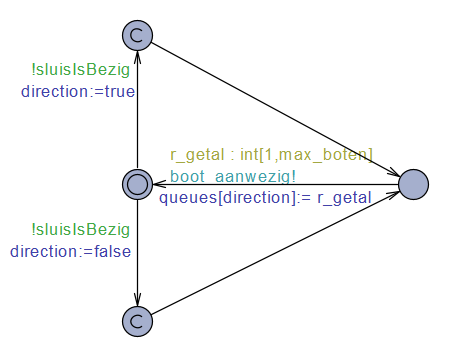
\includegraphics{Request.PNG}
    \caption{Request handler}
    \label{fig:figure1}
    \end{figure}
  
%   [width=10cm, height=10cm] als je de grootte wilt aanpassen

% ---------------afbeelding--van---deur_check-------------------------------
    \begin{figure}[!h]
    \centering
    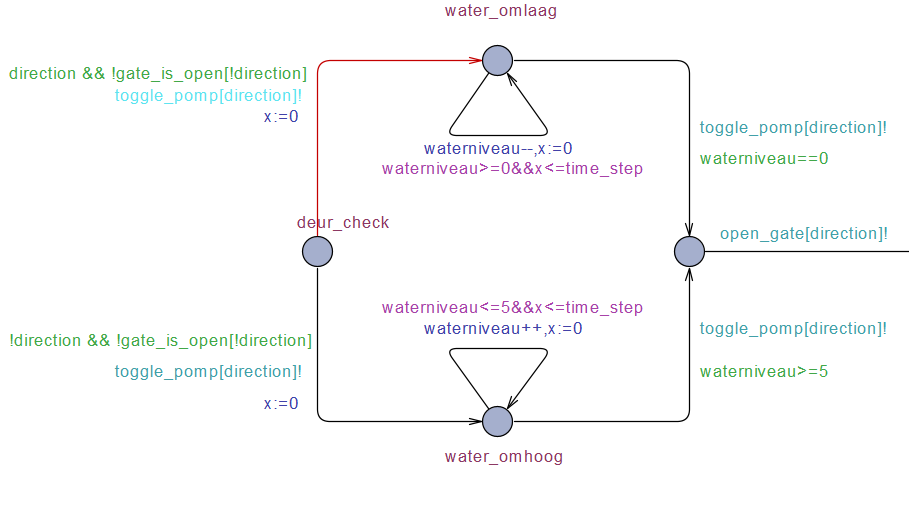
\includegraphics[width=16.5cm, height=9cm]{Deur_Check.PNG}
    \caption{Het waterniveau wordt gereguleerd, Pompen worden aangeroepen}
    \label{fig:figure2}
    \end{figure}

% ---------------------------------Pomp----------------------------------
    \begin{figure}[!h]
    \centering
    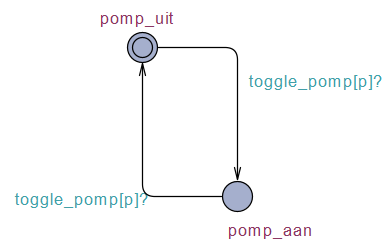
\includegraphics{Pomp.PNG}
    \caption{Pomp in het systeem}
    \label{fig:figure3}
    \end{figure}
    
% ---------------afbeelding--van--Gate-------------------------------
    \begin{figure}[!h]
    \centering
    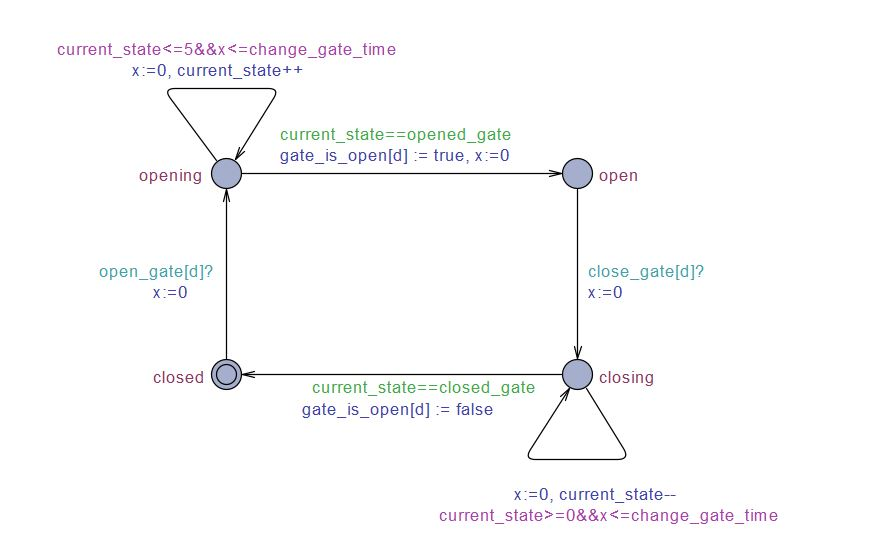
\includegraphics{Gate_final.JPG}
    \caption{Deur in het systeem}
    \label{fig:figure4}
    \end{figure}
    
    
% ----------------------Queue--Legen----------------------------------------------  
    \begin{figure}[!h]
    \centering
    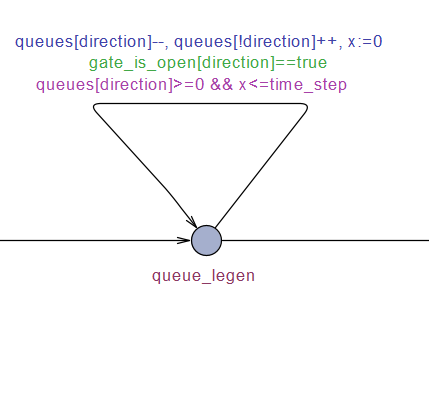
\includegraphics{Queue_Legen.PNG}
    \caption{Queue legen in het systeem}
    \label{fig:figure5}
    \end{figure}
    
% ----------------------Directie----------------------------------------------  
    \begin{figure}[!h]
    \centering
    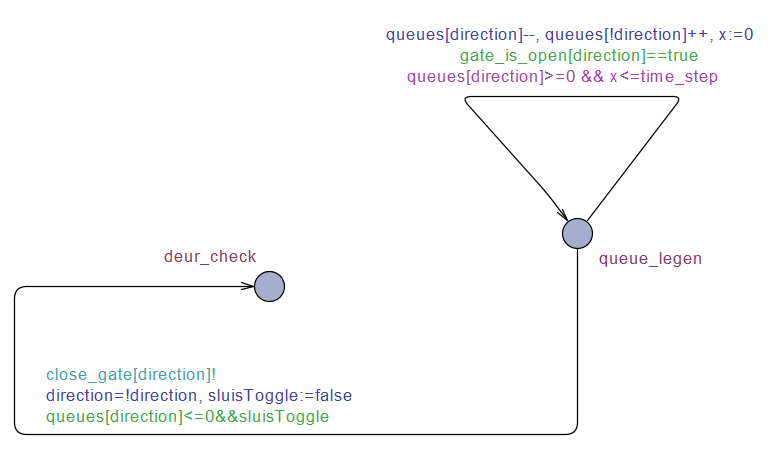
\includegraphics{Directie.PNG}
    \caption{De direction wordt omgedraaid, zodat de sluis de andere kant gaat}
    \label{fig:figure6}
    \end{figure}

% ------------------------------Controller--------------------------------------
    \begin{figure}[!h]
    \centering
    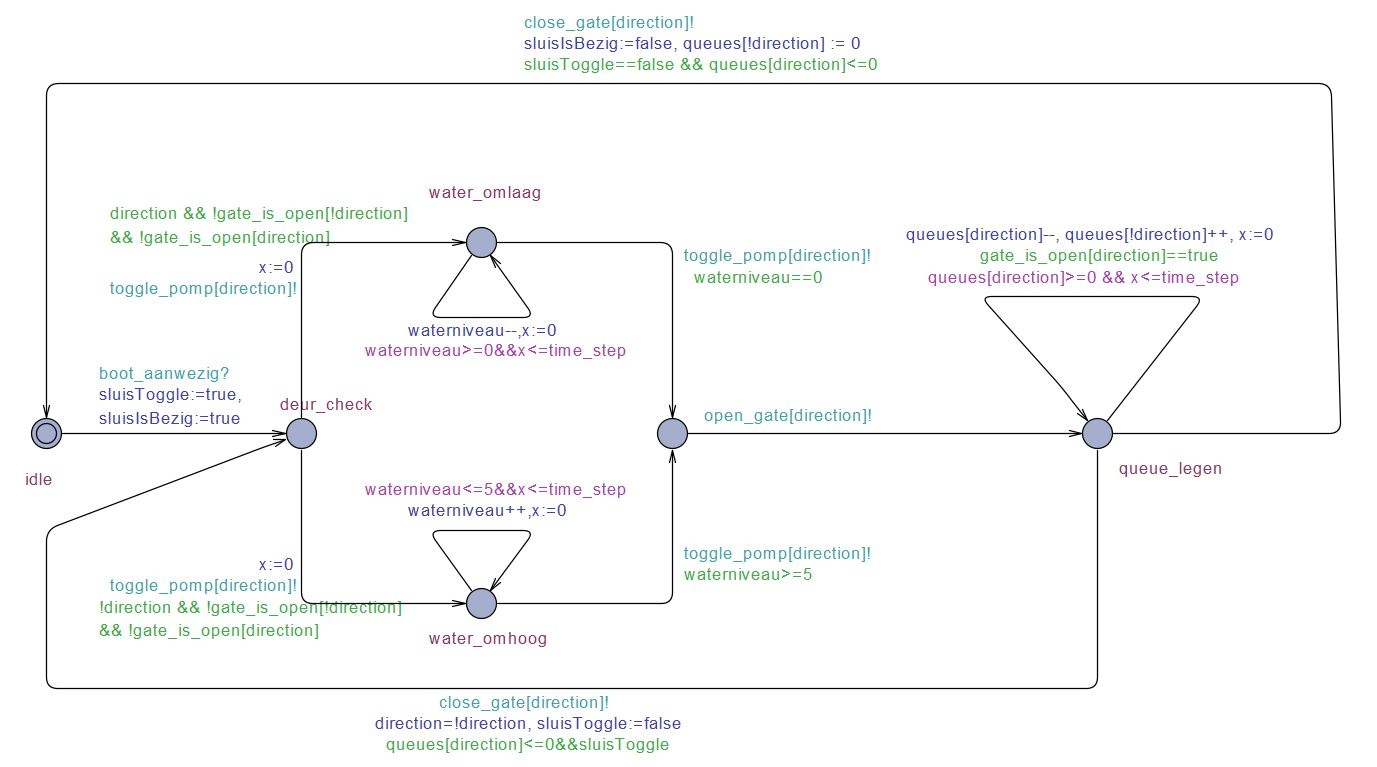
\includegraphics[width=1.6\textwidth, angle=90]{Controller.JPG}
    \caption{Main controller van de sluis}
    \label{fig:figure7}
    \end{figure}
% --------------------------------------------------------------------------------

\newpage
\bibliography{references}
\bibliographystyle{plain}
\end{document}
